\section{The Internet}

\noindent
Terminology and concepts of the internet, which will be used throughout this text.

\begin{Def}[Internet]

    The \textbf{Internet} is a global network of distributed system communicating over an \textbf{Internet Protocol} (IP) \cite{cloudflare_internet_protocol}.
    Documents served over the internet are referred to as \textbf{webpages} or \textbf{websites}.
\end{Def}
\begin{Def}[HTTP \& HTML]

    \textbf{HTTP} (HyperText Transfer Protocol), the protocol which transfer data over the internet, 
    distributing \textbf{HTML} (HyperText Markup Language) documents. Such 
    documents include \textbf{hyperlinks} to other websites, images, and other media \cite{rfc9110}.
\end{Def}
\begin{Def}[RFC (Request for Comments)]

    \textbf{RFC} (Request for Comments) is a publication from the \textbf{Internet Engineering Task Force} (IETF) 
    and the \textbf{Internet Society} (ISOC). This body governs the specifications for the internet and its protocols \cite{rfc}.
\end{Def}

\begin{Def}[DNS and IP Addresses]

    An \textbf{Internet Protocol address} (IP address) is a unique identifier for a device on a network. 
    The \textbf{Domain Name System} (DNS) maps domain names to IP addresses \cite{rfc760}.
\end{Def}

\newpage

\begin{Def}[Web Browser]

    A \textbf{web browser} is a software application for accessing the \textbf{World Wide Web} (WWW) \cite{ou_internet_history}.
\end{Def}

\begin{Def}[URL (Uniform Resource Locator)]

    A \textbf{URL} (Uniform Resource Locator) references each webpage, specifying protocol, domain, and path \cite{w3c_html_href_draft}.
    E.g., \texttt{http://www.example.com/path/to/resource}.
    \begin{itemize}
        \item \textbf{Protocol}: \texttt{http}
        \item \textbf{Domain}: \texttt{www.example.com}
        \item \textbf{Path}: \texttt{/path/to/resource}
    \end{itemize}
\end{Def}
\begin{Def}[Client-Server Model]

    Most of the internet operates on a \textbf{client-server model}, where an agent device\textendash the \textbf{client}\textendash requests data from another agent\textendash the \textbf{server}\textendash 
    which serves an appropriate response. Clients are not servers and vice versa, as they receive and interpret data differently \cite{cloudflare_client_server}.
\end{Def}

\begin{Def}[HTTP Methods]
    
        When a client makes a request to a server, they must specify their intent, categorized by \textbf{HTTP methods} \cite{rfc2616}:
        \begin{itemize}
            \item \textbf{GET}: Retrieve data from the server.
            \item \textbf{POST}: Send data to the server.
            \item \textbf{PUT}: Update data on the server.
            \item \textbf{DELETE}: Remove data from the server.
        \end{itemize}
\end{Def}
\begin{Def}[HTTP Headers]

    \textbf{HTTP headers} are key-value pairs sent between the client and server to provide \textbf{metadata} about the request or response.
    \textbf{Metadata} is data about the transmitted data, telling the receiver how the incoming data should be interpreted \cite{rfc2616}.
\end{Def}


\newpage
\noindent
Tim Berners-Lee and his team at CERN developed the first web server and browser in 1989 \cite{w3c_http_history}.

\begin{table}[h!]
    \centering
    \begin{tabular}{@{}p{3cm}p{10cm}@{}}
    \toprule
    \textbf{HTTP Version} & \textbf{Description} \\ \midrule
    HTTP/0.9 (1991)       & Only supports GET method (retrieving HTML alone). \\
    HTTP/1.0 (1996)       & RFC\#1945, adding support for metadata in HTTP headers, status codes, and POST and HEAD methods \cite{rfc1945}. \\
    HTTP/1.1 (1997)       & Defined in RFC\#2068 and later updated by RFC\#2616, introduced persistent connections, chunked transfer encoding, and additional cache control mechanisms \cite{rfc2068}\cite{rfc2616}. \\
    HTTP/2 (2015)         & RFC\#7540, improving performance by enabling request and response multiplexing, header compression, and prioritization \cite{rfc7540}. \\
    HTTP/3 (2022)         & Builds upon HTTP/2's features and uses the QUIC transport protocol to reduce latency and improve security. \cite{rfc9114} \\ \bottomrule
    \end{tabular}
    \caption{Evolution of HTTP Versions}    
    \label{tab:http_versions}
\end{table}

\begin{Note}
    \textbf{Note:} In short, \textbf{Persistent Connections} allow multiple requests and responses to be sent over a single connection, reducing latency and improving performance \cite{rfc2616}.
    \textbf{Chunked Transfer Encoding} allows the server to send data in chunks, enabling the client to start processing data before the entire response is received \cite{rfc2616}.
    \textbf{Multiplexing}, is the ability to send multiple requests and responses over a single connection, reducing latency and improving performance \cite{multiplexing_networkencyclopedia}. 
     \textbf{QUIC} will be discussed alter on with other transfer protocols in a later section.

\end{Note}

\section{Data Transmission}
This section details how internet traffic is transmitted between devices.
\begin{Def}[ISO Model]

    The \textbf{ISO model} (International Organization for Standardization) is a conceptual framework for transmitted data between devices. 
    It is divided into seven layers of function\cite{ibm_osi_model}. Published in 1984 by the International Organization for Standardization (ISO) \cite{kanade_osi_model}.

\end{Def}
\begin{Def}[TCP/IP Model]

    The \textbf{TCP/IP model} (Transmission Control Protocol/Internet Protocol)
    is a concise representation of the ISO model used in practical settings \cite{yasar_tcpip}.
\end{Def}

\newpage


\begin{Def}[ISO Layers]

    \begin{enumerate}
        \item \textbf{Physical}: Converts data into physical signals (e.g., electrical, optical, or radio waves) for transmission across the network medium (e.g., cables, fiber optics, or wireless channels).
        \item \textbf{Data Link}: local delivery of directly connected devices within \textbf{Local Area Networks} (LAN) using \textbf{Media Access Control} (MAC) addresses for 
        addressing.
        \item \textbf{Network}: Handles addressing, routing, in external networks from source to destination.
        \item \textbf{Transport}: Ensures end-to-end delivery, via a message delivery protocol.
        \item \textbf{Session}: Initiates and terminates network connections, ensuring efficient resource usage.
        \item \textbf{Presentation}: To translate, compress, and encrypt data  (e.g., Operating Systems).
        \item \textbf{Application}: User facing services such as, HTTP , FTP, DNS, SMTP, etc.
    \end{enumerate}
    \hfill \cite{leonard_osi_model}\cite{Rayes2022}
\end{Def}

\begin{Note}
    \textbf{Note:} Many of the above layers are closely related, if not identical. 
    In practice, layers 5-6 are integrated into layer 7, and 
    layers 1-2 are often combined into a single layer in the TCP/IP model.
    
\end{Note}


\begin{Def}[TCP/IP Layers]

    \begin{enumerate}
        \item \textbf{Network Interface}: Physical and data link layers from ISO. 
        \item \textbf{Internet}: Attaches IP addresses to data packets for routing across the internet.
        \item \textbf{Transport}: Defines the delivery protocol, segmenting data into packets.
        \item \textbf{Application}: The Session, Presentation, and Application layers from ISO.
    \end{enumerate}
    \hfill \cite{Rayes2022}
\end{Def}

Despite the numbering of the layers, the user interacts with the application layer, which communicates down the chain
of layers to the physical layer, where the data is transmitted over the network medium. The receiving device then 
interprets the data, moving back up the chain to the application layer.

\newpage 

\noindent
To illustrate the contrast between the ISO and TCP/IP models, consider the diagram:
\begin{figure}[h!]
    \centering
    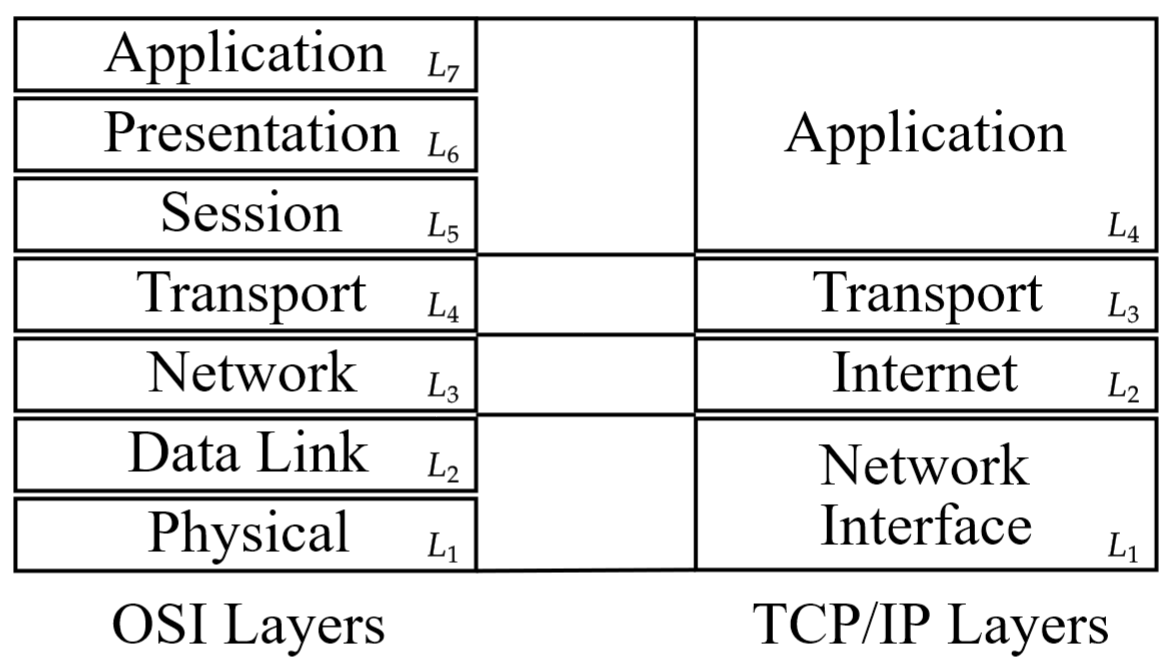
\includegraphics[width=0.7\textwidth]{Sections/network/osi_tcp.png}
    \caption{ISO vs TCP/IP Model}
    \label{fig:osi_tcpip}
\end{figure}

To illustrate two devices communicating over the internet, consider the diagram:

\section{Routing Networks}

\noindent
When IP addresses began


\begin{Def}[Routing]

    \textbf{Routing} is the process of selecting the best path across networks. 
    Data is segmented into packets, each with a destination address. 
    \textbf{Routers} are devices which forward this data through the network.

    Routers have a \textbf{routing table} which maps to other reachable networks. 
    When a packet arrives, the router checks against its routing table to find the best path.
    \hfill \cite{cloudflare_routing}
\end{Def}

\begin{Def}[Hop-by-Hop \& End-to-End Routing]

    \begin{itemize}
        \item  \textbf{Hop-by-Hop Routing}: When a packet of data is forwarded from one router to the next, a forward decision is called a \textbf{hop}.
        \item \textbf{End-to-End Routing}: The process of sending data from source to destination without intermediate hops.
    \end{itemize}
    \noindent
    It is often rare to see end-to-end routing in modern networks, as data is often forwarded through multiple routers. A target 
    destination may be unreachable from a given router.
    \hfill \cite{heimlicher_e2e_hbh}
\end{Def}

\newpage

\begin{Def}[Routing Protocols]
    
    \begin{itemize}
        \item \textbf{IP} (Internet Protocol): The primary protocol for routing data across the internet.
        \item \textbf{BGP} (Border Gateway Protocol): The protocol for routing data between autonomous systems (AS). 
        an AS is a collection of IP networks and routers under the control of a single entity (e.g., an ISP (Internet Service Provider)).
        These may only connect with each other if they have a mutual agreement. ASes identify themselves to 
        external networks using a unique \textbf{Autonomous System Number} (ASN).
        These are unique 16 bit numbers between 1-65534 or 32 bit numbers between 131072-4294967294 (e.g., \texttt{AS12345}) \cite{cloudflare_autonomous_system}.
        \item \textbf{OSPF} (Open Shortest Path First): A link-state routing protocol used within an AS. Link-state protocols are a set 
        of algorithms which determine the best path, based on the topology of a network graph \cite{kurose_link_state_routing}.
        It is also an \textbf{IGP} (Interior Gateway Protocol), meaning it operates within a single AS. It does so by sending out \textbf{LSAs} (Link State Advertisements) to other routers in the AS.
        Then routers in the system build a \textbf{LSADB} (Link State Advertisement Database) of the network topology. Then a shortest path algorithm is run to determine the best path to each network \cite{certbros_ospf_explained}.
        \item \textbf{RIP} (Routing Information Protocol): One of the oldest distance-vector routing protocols, RIP employs hop count as a routing metric, with a maximum allowable hop count of 15, limiting the size of networks it can support.
        It operates as an \textbf{IGP} within a single AS, periodically broadcasting the entire routing table to neighboring routers every 30 seconds,
        which can lead to slower convergence and higher bandwidth usage compared to more advanced protocols.
        Due to these limitations, RIP is generally used in smaller networks and has largely been supplanted by more efficient protocols like OSPF and EIGRP in larger, more complex networks \cite{javatpoint_rip_protocol}.
    \end{itemize}
\end{Def}

\begin{Def}[IP Addressing]

    \textbf{IP addresses} are unique identifiers for devices on a network. 
    There are two versions of IP addresses, \textbf{IPv4} and \textbf{IPv6}.
    IPv4 A 32-bit address, employed since 1983 with a maximum of $2^{32}$ addresses, quickly exhausted all available addresses by the 2010s \cite{info12060246}.
    IPv6 is a 128-bit address, introduced in 1998, with a maximum of $2^{128}$ addresses, in an attempt to address this shortage \cite{deering_ipv6_specification}.
    For example,
    \begin{itemize}
        \item \textbf{IPv4}: \texttt{192.168.1.1} (Decimal Representation)
        \item \textbf{IPv6}: \texttt{2001:0db8:85a3:0000:0000:8a2e:0370:7334} (Hexadecimal Representation)
    \end{itemize}
    \noindent
\end{Def}

\newpage


\begin{Def}[Subnets]

    Instead of a large monolith network of routers, networks can be divided into 
    smaller networks called \textbf{subnets}. I.e., Instead of passing data to every device on a network, routers forward data to a representative device on each subnet.
\end{Def}
    



